\chapter{Novelty Detection}\label{chap:novelty-intro}

This chapter presents a statis

Laying down base concepts that are then used in \autoref{chap:novelty} to
implement novelty detection on the semantic spatial representation.

It start by presenting a brief overview on novelty detection.

It introduces novelty as a 

Shows novelty has an associated ordering.
Shows novelty has a threshold function.


At last a practical example using semantic data and probabilistic graphical
models is presented: it shows how to use the introduced ratio to obtain a
novelty detection system and analyses the performance impact by obtaining more
data and by using an approximation on the unconditional probability.


\begin{itemize}
\item Introduction
\item History
\item Approaches to Novelty Detection
\end{itemize}

\section{Novelty Detection Review and Related Work}
% Introduce novelty detection
Novelty detection deals with detecting that a new input was generated by a class
other than the ones the system knows about~\cite{markou2003novelty}.
It is harder than classification as only positive samples of a class are available
rendering normal classification methods invalid.

Adding capabilities to an agent to detect novel samples allows to increase its
reliability. Novelty signal can then be interpreted by the system to proceed
with more caution as its knowledge does not correctly describe reality.

% Explain threshold approach to novelty detection
Due to the desire of robustness, a novelty detection system is often given the option
to classify non-novel samples as novel. This is implemented as a threshold that describes a trade
between error and rejection: the more the system tries to reduce rejection, the more
prone to produce errors it becomes.



\section{Novelty Detection as a Threshold}
When dealing with a statistic point of view, noisy data or unstable features,
a decision to classify a sample $n$ as novel has an associated error probability
$P(\overline{novel}|n)$.
Accordingly, on a system that classifies a set of inputs $N$ as novel, the
probability of incorrectly classifying a sample as novel is given by the
equation:

\begin{equation}
\label{eq:false-positive}
P(\textnormal{false positive}|\textnormal{positive}) = \frac{\sum_{n \in N}{P(\overline{novel}|n)P(n)}}{\sum_{n \in N}{P(n)}}
\end{equation}

Therefore any novelty system that decides to acknowledge a sample
$a$ as novel should also detect novelty on any sample $b$ satisfying
$P(\overline{novel}|b) < P(\overline{novel}|a)$.
As that always reduce the error probability described in
\autoref{eq:false-positive} as shown:

\begin{equation}
\textnormal{Proof: to be optimal any system accepting }a\textnormal{ should also accept }b
\end{equation}

For the sake of completeness its show here that it also reduces the probability
of false negatives.

\begin{equation}
P(\textnormal{false negative}|\textnormal{negative}) = \frac{\sum_{n \notin N}{P(novel|n)P(n)}}{\sum_{n \notin N}{P(n)}}
\end{equation}


Based on this, it can be said that an optimal novelty detection system is
interested in defining an order relation on all the possible inputs equivalent
to the order defined by the error rate: $P(\overline{novel}|x)$.
And any optimal detector can be described by the largest $P(\overline{novel}|x)$
accepted by it. Which is seen as threshold.


\section{Conditional and Unconditional Probability Ratio}

On the previous section it was shown that an optimal novelty detector can be
implemented with a threshold on top of the order-relation defined by
$P(\overline{novel}|x)$ over $x$. Performing some manipulations with
Bayes theorem and assuming a constant $P(\overline{novel})$ a more usable
form can be attained:

\begin{equation}
\label{eq:novelty-ratio}
          P(\overline{novel}|x)
  =       \frac{P(x|\overline{novel}) P(\overline{novel})}{P(x)}
  \propto \frac{P(x|\overline{novel})}{P(x)}
\end{equation}

Since there is only interest in maintaining the same order-relation as
$P(\overline{novel}|x)$ the absolute value is not needed and any constant
factor can be dropped. Leaving a ratio between a \emph{conditional} and
\emph{unconditional probabilities} suitable for implementing novelty detection
via  thresholding.



\subsection{Conditional Probability}
The conditional probability $P(x|\overline{novel})$ describes the distribution
of the non-novel samples. In case the labelled data available for the agent
to learn a concept comes from this same distribution the correct approach
is to use it as prior-information for modelling the conditional probability.

Note that it is important for the labelled data to come from the same
distribution as where the system will run, as otherwise it will contain some
bias (for example introduced by an incorrect filtering)

Therefore the correct approach is to try to model it 


\subsection{Unconditional Probability}
The unconditional probability $P(x)$ plays an important role on obtaining a
correct order relation for performing novelty detection.
It serves as a normalizing component that allows the system to  whether
a given sample conditional probability arises from it belonging to the
known concept or from it likelihood of being sampled.


On lack of any information about the unconditional probability and conforming to
the principle of maximum entropy (\autoref{sec:max-entropy}) a uniform
distribution must be chosen.
Though, as discussed in \autoref{sec:unlabelled-data}, by using unlabelled data
it becomes possible to obtain prior-information and achieve a better
approximation.


%\subsection{Novelty Detection on a Variable Set of Features}
Note that very often, novelty detection is applied on a fixed set of features
together with an assumption of a uniform unconditional probability.
On those cases $P(x)$ becomes a constant and therefore a novelty threshold
can be directly applied on $P(x|\overline{novel})$ as is the case in \cite{bishop1994novelty}.
But in the case where the set of features $x$ is variable it cannot be
discarded. There $P(x)$ plays a role in levering all the conditional
probabilities on different sets of variables into the same measure units
such that a threshold can be implemented.



\section{A Practical Example}
\label{sec:unlabelled-data}
In order to verify the performance of the proposed threshold functions a synthetic dataset
was generated. To keep it simple only information regarding direct features of
a room were modelled and no structured knowledge such as room connectivity was taken
in account.
The synthetic distribution assumes that an independent and variable size set of features
$x$ is generated by a given room category.
In whole there was 11 different room categories and 7 different measured feature
types. Each feature type can be present more than once in (e.g.: room shape is
extracted from 2D laser scans in more than one position in the room).

The room categories were chosen to mimic as close as possible the real features and
categories existing in reality. And they model different room categories with
different levels of detail. For example: 1 person office, 2 person office, hallway,
robot lab.

From the distribution, 100 labelled samples for 5 of the 11 room categories were
drawn to represent the known concepts and 1000 unlabelled samples were drawn from
all the room categories for learning the unconditional probability distribution.
Using those samples, factors were learnt for the graphs used to model the
conditional distribution and the independent unconditional distribution.
\autoref{fig:simple-experiment} shows the graph structure used for approximate the
trained conditional and unconditional distributions.
Its important to notice that graph $G$ used to model the known classes when given
enough labelled data is able to exactly learn the conditional distribution as it
uses the same structure as the created synthetic distribution.

\begin{figure}[h]
\centering

\subfloat[Graph structure $G$.]{
         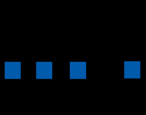
\includegraphics[width=0.27\textwidth]{figures/simple-cond-graph.pdf}}
\qquad
\subfloat[Graph structure $U$.]{
         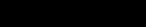
\includegraphics[width=0.27\textwidth]{figures/simple-uniform-graph.pdf}}
\qquad
\subfloat[Graph structure $I$.]{
         
\includegraphics[width=0.27\textwidth]{figures/simple-independent-graph.pdf}}

\caption{\label{fig:simple-experiment}The graph structures used to model the
         conditional and unconditional probability for implementing the novelty
         thresholds $P_G(x)/P_U(x)$ and $P_G(x)/P_I(x)$.}
\end{figure}

% Describe how to obtain the 3 thresholds functions seen on the graphs.
Using the learned models $G$, $U$ and $I$, two thresholds were trained:
$P_G(x)/P_U(x)$ assuming a uniform unconditional distribution
and $P_G(x)/P_I(x)$ assuming an independent unconditional distribution.
Since the distribution is synthetic there is access to $P(x)$ and $P(x|concept)$
and a perfect threshold function could also be created to test how far the
presented thresholds are from optimal.

\subsection{Probability Ratio Comparison}
%%% Results 1
% Show the threshold ratio is an optimal detector (if perfect information was available)
% Show that the thresholds are suitable functions for implementing a static threshold.
As first tryout, the performance of the novelty threshold selection was plotted for a set
of 1000 samples taken out from the whole distribution (\autoref{fig:synthetic-roc}).
Those samples contain different number of sensed properties for each room, mimicking
the dynamic properties expected to see when implemented on a robot.

\begin{figure}[h]
\centering
\includegraphics[width=0.60\textwidth]{results/synthetic-all.pdf}

\caption{\label{fig:synthetic-roc}ROC curve comparing novelty detection performance
         under samples with variable size of sensed properties.}
\end{figure}

The convex shape for the optimal threshold shows that the ratio between conditional
and unconditional probability is indeed an optimal detector and is suitable for
implementing a threshold when the samples are taken from dynamic
distributions (e.g.: some samples where there is only access to room size versus
samples where there is a lot of information about the room properties).

% Discuss importance on approximating unconditional probability.
Its also possible to see how important it is to estimate a correct unconditional
probability in order to obtain a correct novelty measure on the inputs.
The assumption of a uniform unconditional probability has led to very poor results.
That is probably explained by the semantic properties being highly
biased towards some values. And shows that bias plays an important step
in detecting whether a given sensed value is a valuable cue about the room category.



%%% Results 2
% Measure performance of the thresholds as more information becomes available.
\subsection{Performance Changes With Amount of Available Information}
In order to measure the performance impact as more semantic information becomes
available ROC curves were plotted for samples grouped by the number of sensed
semantic features.

\begin{figure}[h]
\centering

\subfloat[3 sensed features]{\includegraphics[width=0.40\textwidth]{results/synthetic-3features.pdf}}
\qquad
\subfloat[5 sensed features]{\includegraphics[width=0.40\textwidth]{results/synthetic-5features.pdf}}

\subfloat[10 sensed features]{\includegraphics[width=0.40\textwidth]{results/synthetic-10features.pdf}}
\qquad
\subfloat[50 sensed features]{\includegraphics[width=0.40\textwidth]{results/synthetic-50features.pdf}}

\caption{\label{fig:synthetic-roc-breakdown}ROC curves plotted showing performance of the
         presented novelty detection method on graphs generated for different amount of
         sensed features.}
\end{figure}

We can see that as the system gains more semantic information it becomes easier
to detect novelty. The input space size increases and allows the several existing
classes to become more easily distinguished.

The performance of the independent threshold decreases as the number of sensed
features increases. This is easily explained by the fact that the graph $I$ is not
able to model the existent dependence between the features. This becomes obvious
as the number of features increases (e.g.: graph $I$ perfectly models $P(x)$ in the
case where only 1 feature is sensed).

The uniform threshold shows a poor performance specially on small size samples
where its performs almost no better than random.
It performance increases as the size of sensed features increases but nonetheless
its very small when compared to how optimal a threshold could be.



